\begin{figure}[htbp]
\centering
\resizebox{\textwidth}{!}{%
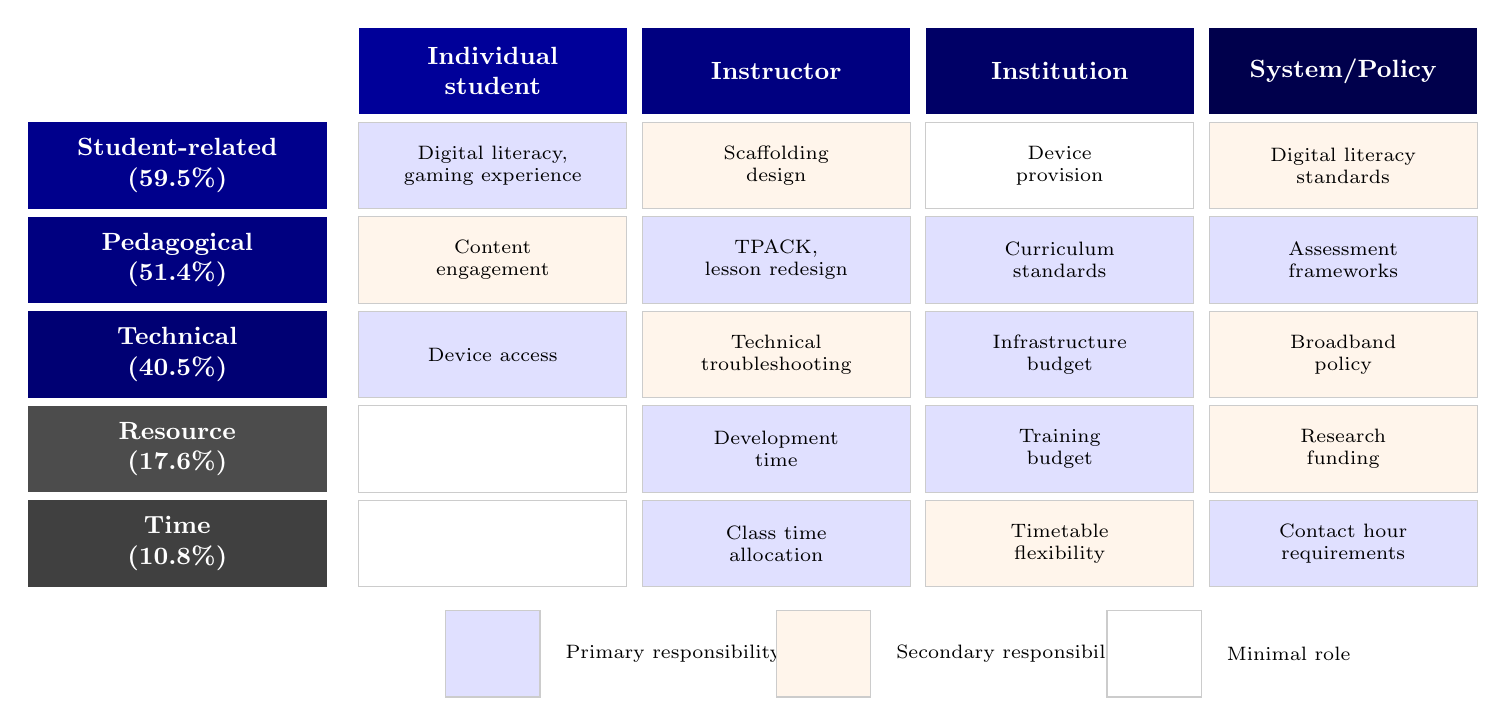
\begin{tikzpicture}[
  hdr/.style={font=\small\bfseries, text=white, minimum height=1.1cm,
    minimum width=3.4cm, align=center},
  rhdr/.style={font=\small\bfseries, text=white, minimum height=1.1cm,
    minimum width=3.8cm, align=center, anchor=east},
  cell/.style={rectangle, draw=gray!40, minimum height=1.1cm,
    minimum width=3.4cm, align=center, font=\scriptsize},
  prim/.style={cell, fill=blue!12},
  sec/.style={cell, fill=orange!8},
  min/.style={cell, fill=white},
]

% Column headers
\node[hdr, fill=blue!60!black] at (0, 0) {Individual\\student};
\node[hdr, fill=blue!50!black] at (3.6, 0) {Instructor};
\node[hdr, fill=blue!40!black] at (7.2, 0) {Institution};
\node[hdr, fill=blue!30!black] at (10.8, 0) {System/Policy};

% Row 1: Student-related (59.5%)
\node[rhdr, fill=blue!55!black] at (-2.1, -1.2) {Student-related\\(59.5\%)};
\node[prim] at (0, -1.2) {Digital literacy,\\gaming experience};
\node[sec] at (3.6, -1.2) {Scaffolding\\design};
\node[min] at (7.2, -1.2) {Device\\provision};
\node[sec] at (10.8, -1.2) {Digital literacy\\standards};

% Row 2: Pedagogical/Curriculum (51.4%)
\node[rhdr, fill=blue!50!black] at (-2.1, -2.4) {Pedagogical\\(51.4\%)};
\node[sec] at (0, -2.4) {Content\\engagement};
\node[prim] at (3.6, -2.4) {TPACK,\\lesson redesign};
\node[prim] at (7.2, -2.4) {Curriculum\\standards};
\node[prim] at (10.8, -2.4) {Assessment\\frameworks};

% Row 3: Technical (40.5%)
\node[rhdr, fill=blue!45!black] at (-2.1, -3.6) {Technical\\(40.5\%)};
\node[prim] at (0, -3.6) {Device access};
\node[sec] at (3.6, -3.6) {Technical\\troubleshooting};
\node[prim] at (7.2, -3.6) {Infrastructure\\budget};
\node[sec] at (10.8, -3.6) {Broadband\\policy};

% Row 4: Resource (17.6%)
\node[rhdr, fill=gray!60!black] at (-2.1, -4.8) {Resource\\(17.6\%)};
\node[min] at (0, -4.8) {};
\node[prim] at (3.6, -4.8) {Development\\time};
\node[prim] at (7.2, -4.8) {Training\\budget};
\node[sec] at (10.8, -4.8) {Research\\funding};

% Row 5: Time (10.8%)
\node[rhdr, fill=gray!50!black] at (-2.1, -6.0) {Time\\(10.8\%)};
\node[min] at (0, -6.0) {};
\node[prim] at (3.6, -6.0) {Class time\\allocation};
\node[sec] at (7.2, -6.0) {Timetable\\flexibility};
\node[prim] at (10.8, -6.0) {Contact hour\\requirements};

% Legend
\node[prim, minimum width=1.2cm] at (0, -7.4) {};
\node[font=\scriptsize, anchor=west] at (0.8, -7.4) {Primary responsibility};
\node[sec, minimum width=1.2cm] at (4.2, -7.4) {};
\node[font=\scriptsize, anchor=west] at (5.0, -7.4) {Secondary responsibility};
\node[min, minimum width=1.2cm] at (8.4, -7.4) {};
\node[font=\scriptsize, anchor=west] at (9.2, -7.4) {Minimal role};

\end{tikzpicture}%
}% end resizebox
\caption{Implementation barrier--stakeholder responsibility matrix. The most frequently reported barriers (student-related, pedagogical) require systemic responses, while the most frequently \textit{addressed} barriers (technical) are tractable at the individual level --- revealing a response mismatch in the literature.}
\label{fig:barrier-stakeholder-matrix}
\end{figure}
